\documentclass[letterpaper]{article}
\usepackage[submission]{aaai2027}
\usepackage[hyphens]{url}
\usepackage{graphicx}
\urlstyle{rm}
\def\UrlFont{\rm}
\usepackage{natbib}
\usepackage{caption}
\frenchspacing
\usepackage{amsmath}
\usepackage{amssymb}
\usepackage{booktabs}
\usepackage{xcolor}
\usepackage{pgfplots}
\usetikzlibrary{arrows.meta}
\pgfplotsset{
    compat=1.18,
    expplot/.style={
        width=\columnwidth,
        tick label style={font=\footnotesize},
        xlabel style={font=\footnotesize},
        ylabel style={font=\footnotesize},
        legend style={font=\footnotesize, draw=none},
        every axis plot/.append style={thick, mark size=2.5pt},
        tick style={black},
        axis line style={black},
    },
}

% Tableau 10 colors
\definecolor{tab-blue}{HTML}{4E79A7}
\definecolor{tab-orange}{HTML}{F28E2B}
\definecolor{tab-red}{HTML}{E15759}
\definecolor{tab-teal}{HTML}{76B7B2}
\definecolor{tab-green}{HTML}{59A14F}
\definecolor{tab-gray}{HTML}{BAB0AC}
\definecolor{lr-blue}{HTML}{78A6D6}
\definecolor{lr-red}{HTML}{F08080}

\newcommand{\acc}{\textsc{Acc}}
\newcommand{\con}{\textsc{Con}}
\newcommand{\ccal}{\textsc{Cal}}
\newcommand{\multirow}[3]{#3}
\pdfinfo{
/TemplateVersion (2027.1)
}
\setcounter{secnumdepth}{0}

\title{Supplementary Material: Position Shortcuts in Reinforcement-Trained LLM Judges}

\author{Anonymous Submission}
\affiliations{}

\begin{document}
\tolerance=1500
\emergencystretch=3em
\hbadness=3000
\maketitle

\section*{Supplementary Material}
This document provides additional training details, data construction information, robustness controls, cross-model results, and extended analyses for the main paper.

\appendix
\section{Training Details}
\label{app:training}

Table~\ref{tab:hparams} lists the shared training hyperparameters used unless otherwise stated.

\textbf{Reward definitions.} The accuracy reward is binary label match: $R_{\text{acc}} = \mathbb{1}[v = v^*]$. The decisiveness reward penalizes ties: $R_{\text{dec}} = \mathbb{1}[v \neq \text{tie}]$. The calibration reward is a Brier-style score over stated confidence: $R_{\text{cal}} = 1 - (c - \mathbb{1}[v = v^*])^2$. The composite reward is $R = \alpha R_{\text{acc}} + \beta R_{\text{dec}} + \gamma R_{\text{cal}}$ with $\alpha = 1.0$, $\beta = 0.5$, and $\gamma = 0.3$.

\begin{table}[htbp]
\centering
\footnotesize
\begin{tabular}{ll}
\toprule
\textbf{Hyperparameter} & \textbf{Value} \\
\midrule
Base model & Qwen2.5-7B-Instruct \\
LoRA rank / $\alpha$ & 64 / 128 \\
Target modules & q, k, v, o projections \\
GRPO group size & 8 \\
Batch size & 4 (grad accum 4) \\
Learning rate & $5 \times 10^{-6}$ (default) \\
LR scheduler & Cosine decay \\
Max prompt / response & 2048 / 1024 tokens \\
Training steps & 500 \\
Reward weights & 1.0, 0.5, 0.3 \\
Seeds & 42, 123, 456, 789 \\
Hardware & 1$\times$ H200 (143GB) per run \\
Training time & $\sim$2.5h per run \\
\bottomrule
\end{tabular}
\caption{Training hyperparameters. Only reward weights and learning rates differ across conditions. For the learning rate study, we additionally test $1 \times 10^{-5}$, $3 \times 10^{-6}$, $2 \times 10^{-6}$, and $1 \times 10^{-6}$.}
\label{tab:hparams}
\end{table}

\clearpage

\section{Data Construction}
\label{app:data}

RewardBench~\citep{lambert2024rewardbench} provides 2,985 preference pairs with gold labels across four domains: chat, reasoning, safety, and coding. We split into 2,089 training, 447 validation (used for early stopping and hyperparameter selection), and 449 test instances using a 70/15/15 stratified split. In our unbalanced judge-prompt conversion, the \texttt{chosen} field is rendered as Response A for 100\% of instances in all splits.

For unbalanced training, we use this data as-is. For balanced training, we include both orientations of each training pair: the original instance with gold label A and a swapped mirror with gold label B. This yields 4,178 balanced training prompts and ensures that position A is preferred in exactly half the training instances. We also run a non-duplicated balanced control with 2,089 prompts in Appendix~\ref{app:dose}.

\textbf{Position bias in preference-data conversion.} The ``always A'' artifact is not unique to RewardBench conversion. We audited multiple widely-used preference datasets and their field formats (Table~\ref{tab:dataset_audit}):

\begin{table}[htbp]
\centering
\footnotesize
\setlength{\tabcolsep}{2pt}
\begin{tabular}{lrcl}
\toprule
\textbf{Dataset} & \textbf{Size} & \textbf{Naive A-rate} & \textbf{Format} \\
\midrule
RewardBench & 2,985 & 100\% & chosen/rejected \\
HH-RLHF & 160,800 & 100\% & chosen/rejected \\
UltraFeedback & 63,967 & varies & completions list \\
PKU-SafeRLHF & 73,907 & 50\% & randomized IDs \\
\bottomrule
\end{tabular}
\caption{Position artifact audit. Datasets using the \texttt{chosen}/\texttt{rejected} convention store the preferred response in a dedicated \texttt{chosen} field. A naive conversion that renders \texttt{chosen} as Response A inherits a 100\% position-label confound.}
\label{tab:dataset_audit}
\end{table}

Datasets following the Anthropic HH-RLHF format~\citep{bai2022training} structurally expose preferred and dispreferred responses through \texttt{chosen}/\texttt{rejected} fields. When converted to pairwise judge training data with ``Response A'' and ``Response B'' labels, the preferred response defaults to position A unless explicit randomization is applied. Our balanced data construction is a general-purpose fix for this conversion pattern.

For SFT experiments, we construct supervised targets by pairing each judge prompt with a gold output that contains a brief rationale followed by the correct verdict in the format ``[[A]]'' or ``[[B]]''. The rationale is generated by the base model and filtered for correct verdict match. For DPO, we construct preference pairs where the chosen output contains the correct verdict and the rejected contains the opposite.

\textbf{SFT 100\% accuracy sanity check.} The SFT result (100\% accuracy, 0\% consistency on unbalanced data) is extreme but expected. The SFT targets encode the correct verdict directly. In unbalanced data, this is always ``[[A]].'' The model learns to always output ``[[A]]'' because that is the only pattern in its training targets. This is the same position confound operating through supervised learning rather than RL: the model memorizes the positional regularity in the gold outputs. The rationales do not contain position-encoding artifacts (they are content-based and filtered for quality), but the verdict labels themselves are the confound. Balanced SFT breaks this: with 50\% ``[[A]]'' and 50\% ``[[B]]'' targets, the model must learn content-based judgment to predict the correct verdict.

For evaluation, we always test both the original and position-swapped version of each test instance, using the swap rate as our consistency metric.

\section{Prompt Template}
\label{app:prompt}

{\small
\begin{verbatim}
You are an expert judge. Given a user 
query and two AI responses, evaluate 
which response is better.

[Query] {query}
[Response A] {response_a}
[Response B] {response_b}

Provide your analysis, then give your 
verdict and confidence in the format:
[[winner, confidence]]
where winner is A, B, or tie, and 
confidence is a number between 0 and 1.
\end{verbatim}
}

\textbf{Output parsing and format handling.} We extract the verdict and confidence from the model's output using a regex matching \texttt{[[winner, confidence]]}. If the output does not match the expected format, we treat it as a parse failure and assign the response as incorrect for accuracy and inconsistent for swap testing. Parse failure rates are below 3\% for Qwen2.5-7B and below 5\% for Qwen3-8B (with thinking disabled). For calibration rewards during training, parse failures receive zero reward. Ties are treated as self-consistent (a model predicting ``tie'' on both orderings is position-invariant). A stricter tie-as-inconsistent check changes the key trained-model consistency comparisons by at most about one point and does not alter the conclusions.

\section{Prompt and Label Controls}
\label{app:label_controls}

Prompt-level mitigation (``evaluate based on content quality only; ordering is random'') only marginally changes consistency: Qwen2.5 moves from 61.7\% to 63.9\%, while Mistral moves from 20.0\% to 18.9\%. We also evaluate unbalanced-GRPO models with alternative label schemes: ``Response 1/2'' and ``Response Left/Right.'' The shortcut persists across all prompt and label variants and all three model families we test (Table~\ref{tab:labels}). Zero parse failures confirm that the Qwen2.5 and Mistral models follow the relabeled format rather than reverting to ``[[A]].'' For Qwen3, the reported prompt/label-control runs use thinking disabled and retain parse failures below 1.3\%; without this setting, parse failures rise to 39--42\% and the control is not interpretable.

\begin{table}[htbp]
\centering
\scriptsize
\setlength{\tabcolsep}{3pt}
\begin{tabular}{@{}llrrrr@{}}
\toprule
\textbf{Model} & \textbf{Control} & \textbf{Acc} & \textbf{Con} & \textbf{Orig.} & \textbf{Parse} \\
\midrule
\multirow{4}{*}{Qwen2.5} & A/B & 94.0 & 61.7 & 94.0 & 0.0 \\
& Anti & 93.8 & 63.9 & 93.8 & 0.0 \\
& 1 / 2 & 94.7 & 60.8 & 94.7 & 0.0 \\
& L/R & 94.2 & 59.9 & 94.2 & 0.0 \\
\midrule
\multirow{4}{*}{Qwen3} & A/B & 88.4 & 78.8 & 88.4 & 1.1 \\
& Anti & 88.0 & 80.2 & 88.0 & 0.7 \\
& 1 / 2 & 88.4 & 81.7 & 88.4 & 1.2 \\
& L/R & 85.7 & 83.7 & 85.7 & 1.0 \\
\midrule
\multirow{4}{*}{Mistral} & A/B & 98.9 & 20.0 & 98.9 & 0.0 \\
& Anti & 98.7 & 18.9 & 98.7 & 0.0 \\
& 1 / 2 & 99.6 & 12.0 & 99.6 & 0.0 \\
& L/R & 99.1 & 15.6 & 99.1 & 0.0 \\
\bottomrule
\end{tabular}
\caption{Prompt and label controls. Anti is the ordering-randomized anti-shortcut prompt; L/R denotes Left/Right labels. Orig. is original-order first-selection; Parse is the two-order parse-failure rate.}
\label{tab:labels}
\end{table}

\section{Evaluation-Time Swap Filtering}
\label{app:posthoc}

Post-hoc swap filtering can identify examples on which the original and swapped predictions disagree, but it does not repair the underlying model on those examples. We keep only pairs whose predictions are logically consistent after swapping positions. This produces a high-accuracy retained subset, but coverage collapses exactly when the shortcut is severe: unbalanced SFT retains 0.0\% of examples, and unbalanced full GRPO retains only 58.7\% (Table~\ref{tab:posthoc}). A random fallback on discarded examples reduces unbalanced full GRPO to 74.9\% expected accuracy, while balanced full GRPO keeps 84.0\% coverage and 82.6\% expected fallback accuracy. Thus swap filtering is useful as a diagnostic or selective abstention rule, but data balancing addresses the source of the shortcut.

\begin{table}[htbp]
\centering
\scriptsize
\setlength{\tabcolsep}{3pt}
\begin{tabular}{@{}lrrrr@{}}
\toprule
\textbf{Setting} & \textbf{Acc} & \textbf{Cov.} & \textbf{Ret.} & \textbf{Rand.} \\
\midrule
Baseline & 80.2 & 81.5 & 84.2 & 77.8 \\
SFT unbal & 100.0 & 0.0 & -- & 50.0 \\
SFT bal & 91.3 & 87.1 & 96.2 & 90.2 \\
GRPO-A unbal & 94.7 & 59.8 & 92.4 & 75.3 \\
GRPO-F unbal & 94.7 & 58.7 & 92.3 & 74.9 \\
GRPO-F bal & 83.7 & 84.0 & 88.8 & 82.6 \\
\bottomrule
\end{tabular}
\caption{Post-hoc swap filtering on Qwen2.5. Cov. is retained coverage; Ret. is accuracy on retained examples; Rand. assumes a random binary fallback on discarded examples. GRPO rows report seed means.}
\label{tab:posthoc}
\end{table}

\section{Length-Confound Control}
\label{app:length}

To separate position shortcuts from generic shortcut learning, we include a non-positional confound control in which the training preference is correlated with response length rather than response order. This control does not produce the same failure mode: length-confounded GRPO remains close to the untrained baseline in both consistency and first-position selection (Table~\ref{tab:length}). In contrast, position-confounded GRPO-A increases original-order accuracy to 94.7\% while reducing consistency to 59.8\% and pushing first-position selection to 68.1\%. This suggests that the severe collapse we study is tied to the globally predictive position feature introduced by preference-data conversion, not simply to the presence of any spurious training feature.

\begin{table}[htbp]
\centering
\scriptsize
\setlength{\tabcolsep}{3pt}
\begin{tabular}{@{}lrrrr@{}}
\toprule
\textbf{Setting} & \textbf{Acc} & \textbf{Swap} & \textbf{Con} & \textbf{First} \\
\midrule
Baseline & 80.2 & 75.3 & 81.5 & 49.3 \\
Position-conf. GRPO-A & 94.7 & 55.7 & 59.8 & 68.1 \\
Length-conf. GRPO & 80.9 & 75.8 & 79.7 & 50.6 \\
\bottomrule
\end{tabular}
\caption{Length-confound control on Qwen2.5. Swap is swapped-order accuracy; First is the two-order first-position selection rate. The two GRPO rows report three-seed means.}
\label{tab:length}
\end{table}

\section{Cross-Model Validation}
\label{app:crossmodel}

To verify that our findings generalize beyond a single model family, we replicate experiments on Qwen3-8B~\citep{qwen2025qwen3} (a newer-generation Qwen model) and Mistral-7B-Instruct-v0.3~\citep{jiang2023mistral} (a completely different architecture and pre-training corpus from Mistral AI). Table~\ref{tab:crossmodel} reports the full cross-model comparison. For Qwen3, we use the disable-thinking baseline run so that parsing behavior matches the rest of the Qwen3 evaluations.

\begin{table}[htbp]
\centering
\footnotesize
\begin{tabular}{llcc}
\toprule
\textbf{Method} & \textbf{Data} & \textbf{Acc} & \textbf{Con} \\
\midrule
\multicolumn{4}{l}{\textit{Qwen2.5-7B-Instruct (primary)}} \\
Baseline & --- & 80.2 & 81.5 \\
SFT & unbal & 100.0 & 0.0 \\
DPO & unbal & 94.2 & 54.3 \\
GRPO & unbal & 94.7{\scriptsize$\pm$0.9} & 58.7{\scriptsize$\pm$9.1} \\
SFT & bal & 91.3 & 87.1 \\
GRPO & bal & 83.7{\scriptsize$\pm$1.1} & 84.0{\scriptsize$\pm$0.8} \\
\midrule
\multicolumn{4}{l}{\textit{Qwen3-8B (cross-generation)}} \\
Baseline & --- & 86.0 & 80.4 \\
SFT & unbal & 100.0{\scriptsize$\pm$0.0} & 0.0{\scriptsize$\pm$0.0} \\
DPO & unbal & 89.3 & 81.3 \\
GRPO & unbal & 88.7{\scriptsize$\pm$0.3} & 80.0{\scriptsize$\pm$1.0} \\
SFT & bal & 88.5{\scriptsize$\pm$1.1} & 89.1{\scriptsize$\pm$0.3} \\
DPO & bal & 88.6 & 85.3 \\
GRPO & bal & 87.4{\scriptsize$\pm$0.8} & 82.2{\scriptsize$\pm$0.6} \\
\midrule
\multicolumn{4}{l}{\textit{Mistral-7B-Instruct-v0.3 (cross-family)}} \\
Baseline & --- & 65.7 & 64.8 \\
SFT & unbal & 100.0 & 0.0 \\
SFT & bal & 92.2 & 84.9 \\
GRPO & unbal & 98.4{\scriptsize$\pm$0.4} & 23.0{\scriptsize$\pm$3.6} \\
GRPO & bal & 81.1{\scriptsize$\pm$0.9} & 68.3{\scriptsize$\pm$3.6} \\
\bottomrule
\end{tabular}
\caption{Cross-model validation across three model families. The position shortcut replicates, but severity is model-dependent: Mistral shows the most extreme collapse, Qwen2.5 is intermediate, and Qwen3 shows the mildest GRPO consistency loss under disable-thinking evaluation.}
\label{tab:crossmodel}
\end{table}

Shortcut severity is model-dependent. Mistral-7B, with the weakest baseline judge ability (65.7\%), is almost completely dominated by the shortcut after training (98.4\% accuracy, 23.0\% consistency). Qwen2.5-7B (baseline 80.2\%) shows a moderate shortcut (94.7\%/58.7\%). Qwen3-8B starts from the strongest original-order baseline (86.0\%) and shows much milder consistency damage under unbalanced GRPO (80.4\% baseline $\to$ 80.0\% unbalanced), while balanced GRPO remains slightly above baseline (82.2\%). The positional feature and content features compete for representational capacity during RL optimization, and the outcome depends on the relative strength of the content signal at initialization. Stronger initial comparison ability can buffer the GRPO shortcut, but it does not remove the risk: unbalanced Qwen3 SFT still collapses to 0.0\% consistency, and aggressive learning rates still reduce consistency. Balanced data is therefore the more reliable fix because it removes the position-label correlation rather than relying on model capacity to resist it.

The severity gradient extends to the \emph{speed} of shortcut emergence. Checkpoint-level evaluation reveals that Mistral-7B is already dominated by step 100 (98.7\% accuracy, 20.3\% consistency, close to its final step-500 values), while Qwen2.5-7B shows gradual degradation through all 500 steps (84.6\%/81.7\% at step 100 $\to$ 94.0\%/61.7\% at step 500). This temporal difference suggests that weaker baseline judge capability may leave less competition against the positional feature. Practically, monitoring Mistral-class judges would need to happen very early, while Qwen-class judges provide a longer window for early stopping or diagnostic intervention.

A flatter learning-rate sensitivity pattern also appears on Qwen3-8B. Consistency stays in the high-70s to low-80s across the Qwen3 sweep (Table~\ref{tab:crosslr}), compared to the sharp Qwen2.5-7B drop at lr=3e-6 (75.7\%) and beyond. The stronger model resists the shortcut at moderate learning rates but still loses consistency at aggressive ones (lr=1e-5: 78.4\% consistency).

\begin{table}[htbp]
\centering
\footnotesize
\begin{tabular}{lcccc}
\toprule
\textbf{LR} & \multicolumn{2}{c}{\textbf{Qwen2.5-7B}} & \multicolumn{2}{c}{\textbf{Qwen3-8B}} \\
\cmidrule(lr){2-3} \cmidrule(lr){4-5}
 & Acc & Con & Acc & Con \\
\midrule
1e-6 & 83.7 & 83.3 & 89.1 & 82.4 \\
2e-6 & 85.7 & 81.1 & 87.8 & 81.5 \\
3e-6 & 90.0 & 75.7 & 87.8 & 82.6 \\
5e-6 & 94.0 & 61.7 & 88.4 & 78.8 \\
1e-5 & 98.9 & 38.1 & 90.2 & 78.4 \\
\bottomrule
\end{tabular}
\caption{Cross-model LR sensitivity. The Qwen2.5 sweep uses the full reward, while the Qwen3 sweep uses the accuracy reward; rows are single-seed controls. The threshold effect is sharper on Qwen2.5-7B (about 45 pp consistency loss across the range) than Qwen3-8B (about 4 pp), but both show lower consistency at aggressive rates.}
\label{tab:crosslr}
\end{table}

Multi-objective rewards also fail to reliably restore consistency on Qwen3-8B: the decisiveness reward raises consistency from 78.8\% to 82.0\%, while the calibration proxy lowers it (78.0\%, below acc-only). The composite reward remains below balanced GRPO under the tested weights. This supports the conclusion that these proxy rewards are insufficient for this data-level confound across the evaluated model generations.

All experiments use NVIDIA H200 GPUs (143GB). Total compute: approximately 200 H200-GPU-hours across all experiments.

\section{External Check on Published RL-Trained Judges}
\label{app:judgelrm}

As an external check, we evaluate JudgeLRM's publicly released checkpoints~\citep{chen2025judgelrm} with the same position-swap diagnostic (Table~\ref{tab:judgelrm}). JudgeLRM-7B achieves 81.3\% original-order accuracy but 66.1\% swap accuracy and 75.7\% consistency, while JudgeLRM-3B achieves 76.8\% original-order accuracy, 55.9\% swap accuracy, and 67.9\% consistency. These results do not imply that all gains in prior judge training are shortcuts; they show that standard accuracy can hide a position-dependent component.

\begin{table}[htbp]
\centering
\scriptsize
\setlength{\tabcolsep}{2.5pt}
\resizebox{\columnwidth}{!}{%
\begin{tabular}{lccccc}
\toprule
\textbf{Model} & \textbf{Orig Acc} & \textbf{Swap Acc} & \textbf{Con} & \textbf{First-pos} & \textbf{Bias} \\
\midrule
JudgeLRM-7B & 81.3 & 66.1 & 75.7 & 53.1 & 13.4 \\
JudgeLRM-3B & 76.8 & 55.9 & 67.9 & 56.7 & 15.4 \\
\bottomrule
\end{tabular}
}
\caption{Published RL-trained judges also show a position-dependent component under the swap diagnostic. Bias is the always-first minus always-second inconsistent rate.}
\label{tab:judgelrm}
\end{table}

\section{Multi-Seed Stability}
\label{app:seeds}

The primary GRPO pattern is stable across random seeds rather than driven by a single run. Table~\ref{tab:seeds} reports individual seed results for representative unbalanced and balanced conditions. Unbalanced runs maintain high original-order accuracy but low consistency and elevated first-position selection; balanced runs keep consistency high and first-position selection near neutral.

\begin{table}[htbp]
\centering
\scriptsize
\begin{tabular}{llccc}
\toprule
\textbf{Method} & \textbf{Seed} & \textbf{Acc} & \textbf{Con} & \textbf{First-pos} \\
\midrule
\multirow{3}{*}{Acc-only unbal} & s1 & 94.4 & 60.8 & 67.4 \\
 & s2 & 95.6 & 51.7 & 72.0 \\
 & s3 & 94.2 & 66.8 & 64.9 \\
\midrule
\multirow{4}{*}{Full unbal} & s1 & 94.0 & 61.7 & 67.4 \\
 & s2 & 96.0 & 45.2 & 75.3 \\
 & s3 & 94.2 & 63.7 & 66.5 \\
 & s4 & 94.4 & 64.4 & 66.1 \\
\midrule
\multirow{5}{*}{Full bal} & s1 & 84.6 & 85.3 & 50.1 \\
 & s2 & 82.2 & 83.7 & 48.6 \\
 & s3 & 84.4 & 83.3 & 51.3 \\
 & s4 & 82.9 & 83.7 & 49.4 \\
 & s5 & 84.4 & 84.0 & 50.3 \\
\bottomrule
\end{tabular}
\caption{Per-seed results for Qwen2.5 GRPO. Balanced training consistently keeps position consistency high and first-position selection near 50\%.}
\label{tab:seeds}
\end{table}

\section{Statistical Uncertainty Checks}
\label{app:uncertainty}

We add local uncertainty checks for the main diagnostic effects (Table~\ref{tab:uncertainty}). For single-run SFT comparisons, we use paired bootstrap resampling over the 449 matched test examples. For multi-seed GRPO comparisons, we bootstrap the available seed means; these intervals are descriptive because the number of seeds is small.

\begin{table}[htbp]
\centering
\scriptsize
\setlength{\tabcolsep}{3pt}
\resizebox{\columnwidth}{!}{%
\begin{tabular}{llcc}
\toprule
\textbf{Comparison} & \textbf{Metric} & \textbf{Diff} & \textbf{95\% CI} \\
\midrule
SFT unbal $\to$ SFT bal & Con & +87.1 & [84.0, 90.0] \\
SFT unbal $\to$ SFT bal & First-pos & -48.9 & [-50.6, -47.2] \\
Baseline $\to$ SFT bal & Acc & +11.1 & [7.6, 14.9] \\
Baseline $\to$ SFT bal & Con & +5.6 & [1.1, 10.0] \\
Qwen2.5 GRPO unbal $\to$ bal & Con & +25.3 & [19.8, 34.4] \\
Qwen2.5 GRPO unbal $\to$ bal & First-pos & -18.9 & [-23.3, -16.0] \\
Qwen3 GRPO unbal $\to$ bal & Con & +2.2 & [1.1, 3.3] \\
Mistral GRPO unbal $\to$ bal & Con & +45.2 & [40.4, 50.1] \\
\bottomrule
\end{tabular}
}
\caption{Bootstrap uncertainty checks. Diff is after $-$ before in percentage points. Single-run SFT rows use paired-instance bootstrap; multi-seed GRPO rows use seed-mean bootstrap.}
\label{tab:uncertainty}
\end{table}

The intervals support the paper's qualitative interpretation without requiring stronger statistical language. The SFT shortcut collapse and recovery are much larger than instance-level uncertainty. For Qwen2.5 and Mistral GRPO, balancing produces large consistency gains and reduces first-position selection. For Qwen3 GRPO, the consistency gain is small but positive under the local seed-mean bootstrap, matching the cross-model conclusion that stronger models show greater shortcut resistance rather than immunity.

\section{Learning Rate Sensitivity}
\label{app:lr}

The complete learning rate data is shown in Table~\ref{tab:lr} and visualized in Figure~\ref{fig:lr}.

\begin{figure}[t]
\centering
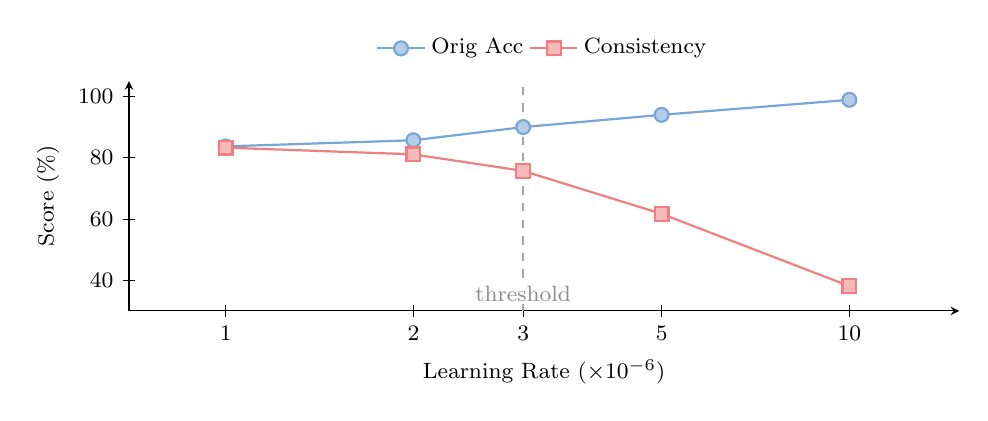
\begin{tikzpicture}
\begin{axis}[
    expplot,
    height=4.5cm,
    xlabel={Learning Rate ($\times 10^{-6}$)},
    ylabel={Score (\%)},
    xmode=log,
    xmin=7e-7, xmax=1.5e-5,
    ymin=30, ymax=105,
    xtick={1e-6, 2e-6, 3e-6, 5e-6, 1e-5},
    xticklabels={1, 2, 3, 5, 10},
    ytick={40,60,80,100},
    grid=none,
    legend style={at={(0.5,1.05)}, anchor=south, legend columns=2},
    axis lines=left,
    clip=false,
]
\addplot[lr-blue, mark=*, mark options={fill=lr-blue!55, draw=lr-blue}] coordinates {(1e-6,83.7) (2e-6,85.7) (3e-6,90.0) (5e-6,94.0) (1e-5,98.9)};
\addlegendentry{Orig Acc}
\addplot[lr-red, mark=square*, mark options={fill=lr-red!55, draw=lr-red}] coordinates {(1e-6,83.3) (2e-6,81.1) (3e-6,75.7) (5e-6,61.7) (1e-5,38.1)};
\addlegendentry{Consistency}
\addplot[black!35, dashed, forget plot] coordinates {(3e-6,30) (3e-6,105)};
\node[font=\footnotesize, anchor=south, text=black!45, fill=white, inner sep=1pt] at (axis cs:3e-6,32) {threshold};
\end{axis}
\end{tikzpicture}
\caption{Learning rate controls shortcut activation. Original-order accuracy rises with optimization pressure, while consistency remains high at conservative rates and then drops sharply once optimization reaches the marked threshold.}
\label{fig:lr}
\end{figure}

\begin{table}[tbp]
\centering
\footnotesize
\begin{tabular}{lccc}
\toprule
\textbf{Learning Rate} & \textbf{Acc} & \textbf{Con} & \textbf{First-pos} \\
\midrule
Baseline & 80.2 & 81.5 & 49.3 \\
1e-6 & 83.7 & 83.3 & 51.0 \\
2e-6 & 85.7 & 81.1 & 54.3 \\
3e-6 & 90.0 & 75.7 & 58.2 \\
5e-6 (standard) & 94.0 & 61.7 & 67.4 \\
1e-5 & 98.9 & 38.1 & 80.5 \\
\bottomrule
\end{tabular}
\caption{Full learning rate sweep. First-position rate increases with training intensity as consistency falls.}
\label{tab:lr}
\end{table}
\section{Training Algorithm Controls}
\label{app:sft}

The position shortcut is not specific to any training paradigm. SFT on unbalanced data achieves 100\% accuracy with 0\% consistency. DPO falls between SFT and GRPO in severity (94.2\%/54.3\%). GRPO retains partial consistency (58.7\% multi-seed mean). The ordering SFT $>$ DPO $>$ GRPO in shortcut severity is consistent with different degrees of implicit regularization, but all three objectives remain vulnerable to the position-label confound.

When given balanced data, SFT achieves higher accuracy (91.3\% vs 84.6\% for GRPO in the corresponding single run), suggesting that it can be more data-efficient when the supervision is deconfounded. SFT's direct likelihood maximization may therefore make it both a strong learner and highly vulnerable to label-position confounds, while GRPO's exploration-based optimization appears to provide partial implicit regularization against shortcuts.

\section{Cross-Model Learning Rate Sensitivity}
\label{app:crosslr}

Figure~\ref{fig:crosslr} shows that learning-rate sensitivity is much flatter on Qwen3-8B, suggesting that the activation point depends on model capability and reward setup.

\begin{figure}[htbp]
\centering
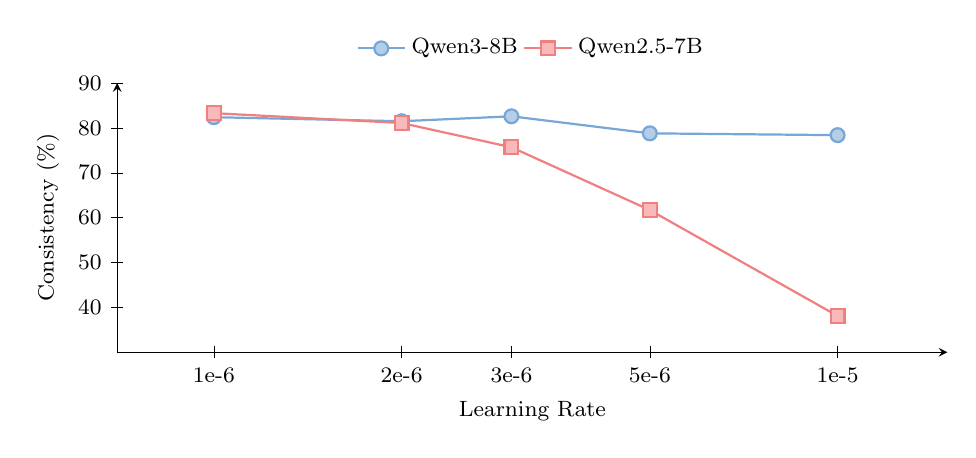
\begin{tikzpicture}
\begin{axis}[
    expplot,
    height=5cm,
    xlabel={Learning Rate},
    ylabel={Consistency (\%)},
    xmode=log,
    xmin=7e-7, xmax=1.5e-5,
    ymin=30, ymax=90,
    xtick={1e-6, 2e-6, 3e-6, 5e-6, 1e-5},
    xticklabels={1e-6, 2e-6, 3e-6, 5e-6, 1e-5},
    ytick={40,50,60,70,80,90},
    grid=none,
    legend style={at={(0.5,1.05)}, anchor=south, legend columns=2},
    axis lines=left,
]
\addplot[lr-blue, mark=*, mark options={fill=lr-blue!55, draw=lr-blue}] coordinates {(1e-6,82.4) (2e-6,81.5) (3e-6,82.6) (5e-6,78.8) (1e-5,78.4)};
\addlegendentry{Qwen3-8B}
\addplot[lr-red, mark=square*, mark options={fill=lr-red!55, draw=lr-red}] coordinates {(1e-6,83.3) (2e-6,81.1) (3e-6,75.7) (5e-6,61.7) (1e-5,38.1)};
\addlegendentry{Qwen2.5-7B}
\end{axis}
\end{tikzpicture}
\caption{Consistency as a function of learning rate for two model generations. Qwen2.5-7B shows a sharp threshold at lr=3e-6, losing about 45 pp of consistency across the range. Qwen3-8B changes by about 4 pp under the available accuracy-reward sweep. Stronger models have higher shortcut resistance but are not immune.}
\label{fig:crosslr}
\end{figure}

The contrast between the two curves suggests an important practical insight: model capability can act as a partial buffer against shortcut learning. Qwen3-8B maintains position-invariant judgment better under moderate optimization pressure. However, at aggressive learning rates, even the stronger model begins to lose consistency. This implies that scaling alone should not be treated as a substitute for auditing the position shortcut.

\section{Multi-Objective Reward Analysis}
\label{app:reward}

A key question is whether reward engineering can substitute for data deconfounding. We test three reward configurations on both models (all on unbalanced data). For Qwen2.5-7B, rows report seed means where available; Qwen3-8B rows are single-seed reward controls.

\begin{table}[htbp]
\centering
\footnotesize
\begin{tabular}{lcccc}
\toprule
\textbf{Reward} & \multicolumn{2}{c}{\textbf{Qwen2.5-7B}} & \multicolumn{2}{c}{\textbf{Qwen3-8B}} \\
\cmidrule(lr){2-3} \cmidrule(lr){4-5}
 & Acc & Con & Acc & Con \\
\midrule
Accuracy only & 94.7 & 59.8 & 88.4 & 78.8 \\
+ Decisive & 93.9 & 66.3 & 88.2 & 82.0 \\
+ Calibration & 95.4 & 56.1 & 89.1 & 78.0 \\
Full composite & 94.7 & 58.7 & 87.8 & 80.8 \\
\bottomrule
\end{tabular}
\caption{Reward ablation across models. Qwen2.5 rows use multi-seed means where available, while Qwen3 rows are single-seed controls. No proxy reward exceeds balanced data (Qwen2.5 GRPO balanced: 84.0\% con, Qwen3 GRPO balanced: 82.2\% con). The calibration proxy lowers consistency on both models.}
\label{tab:reward_ablation}
\end{table}

The tested proxy rewards do not replace data deconfounding (Table~\ref{tab:reward_ablation}). The decisiveness reward improves consistency by penalizing tie hedging, but it cannot distinguish between a model that is decisive because it understands the content and one that is decisive because it follows the position shortcut. The calibration proxy actually \emph{lowers} consistency on both models, because confidence in A is not penalized when the training data always rewards A. Overall, the tested reward components help only partially and do not match the cleaner fix of removing the position-label correlation from the training data.

\section{Training Dynamics Details}
\label{app:dynamics}

Table~\ref{tab:dynamics} gives the paired checkpoint-level data for the training dynamics experiment. At these shared checkpoints, original-order accuracy and first-position selection increase as training proceeds, while consistency is preserved only at the earliest checkpoint and then drops sharply. The composite reward follows the same shortcut trajectory rather than materially slowing the collapse.

\begin{center}
\begin{minipage}{\columnwidth}
\centering
\resizebox{\columnwidth}{!}{%
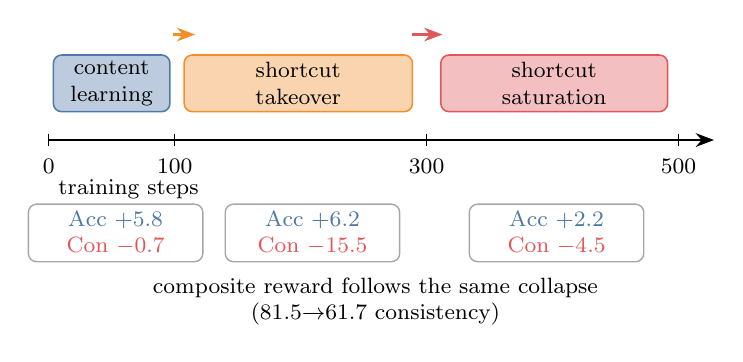
\begin{tikzpicture}[
    font=\footnotesize,
    >=Stealth,
    phase/.style={draw, line width=0.55pt, rounded corners=3pt, align=center, minimum height=0.72cm, inner sep=2pt},
    chip/.style={draw=black!35, fill=white, line width=0.5pt, rounded corners=3pt, align=center, inner sep=2.5pt, text width=2.04cm},
    axis/.style={-Stealth, thick, draw=black}
]
\draw[axis] (0,0) -- (8.45,0);
\foreach \x/\label in {0/0,1.6/100,4.8/300,8.0/500} {
    \draw[black] (\x,0.08) -- (\x,-0.08);
    \node[anchor=north, text=black] at (\x,-0.12) {\label};
}
\node[anchor=west, font=\footnotesize] at (0,-0.62) {training steps};

\draw[draw=tab-blue, fill=tab-blue!38, line width=0.55pt, rounded corners=3pt] (0.06,0.36) rectangle (1.54,1.08);
\draw[draw=tab-orange, fill=tab-orange!38, line width=0.55pt, rounded corners=3pt] (1.72,0.36) rectangle (4.62,1.08);
\draw[draw=tab-red, fill=tab-red!38, line width=0.55pt, rounded corners=3pt] (4.98,0.36) rectangle (7.86,1.08);
\node[align=center] at (0.80,0.72) {content\\learning};
\node[align=center] at (3.17,0.72) {shortcut\\takeover};
\node[align=center] at (6.42,0.72) {shortcut\\saturation};

\node[chip] at (0.85,-1.18) {\textcolor{tab-blue}{Acc $+5.8$}\\\textcolor{tab-red}{Con $-0.7$}};
\node[chip] at (3.35,-1.18) {\textcolor{tab-blue}{Acc $+6.2$}\\\textcolor{tab-red}{Con $-15.5$}};
\node[chip] at (6.45,-1.18) {\textcolor{tab-blue}{Acc $+2.2$}\\\textcolor{tab-red}{Con $-4.5$}};

\draw[->, thick, draw=tab-orange] (1.58,1.34) -- (1.86,1.34);
\draw[->, thick, draw=tab-red] (4.62,1.34) -- (5.00,1.34);
\node[align=center, font=\footnotesize, text=black] at (4.15,-2.05) {composite reward follows the same collapse\\(81.5$\to$61.7 consistency)};
\end{tikzpicture}
}
\captionsetup{hypcap=false}
\captionof{figure}{Training dynamics as phases. Early training improves original-order accuracy with little consistency loss; mid-training is the shortcut takeover window; late training saturates the positional policy.}
\label{fig:dynamics}
\end{minipage}
\end{center}

\begin{center}
\begin{minipage}{\columnwidth}
\centering
\footnotesize
\begin{tabular}{lcccccc}
\toprule
\textbf{Steps} & \multicolumn{3}{c}{\textbf{Acc-only}} & \multicolumn{3}{c}{\textbf{Full}} \\
\cmidrule(lr){2-4} \cmidrule(lr){5-7}
 & Acc & Con & First & Acc & Con & First \\
\midrule
0 (base) & 80.2 & 81.5 & 49.3 & 80.2 & 81.5 & 49.3 \\
100 & 86.0 & 80.8 & 53.8 & 84.6 & 81.7 & 53.5 \\
200 & 89.1 & 76.8 & 57.1 & 90.9 & 74.6 & 59.8 \\
300 & 92.2 & 65.3 & 63.7 & 93.5 & 65.9 & 64.9 \\
500 & 94.4 & 60.8 & 67.4 & 94.0 & 61.7 & 67.4 \\
\bottomrule
\end{tabular}
\captionsetup{hypcap=false}
\captionof{table}{Training dynamics at paired checkpoints. Accuracy and first-position selection increase together, while consistency drops after the earliest checkpoint. The composite reward reaches nearly the same endpoint as the accuracy-only reward.}
\label{tab:dynamics}
\end{minipage}
\end{center}

\section{Per-Domain Analysis}
\label{app:domain}

Each domain's vulnerability to the shortcut varies substantially (Table~\ref{tab:domain}). We report the primary Qwen2.5 GRPO full setting by domain, using seed means for the unbalanced and balanced rows. The shortcut appears in every domain, but reasoning shows the cleanest collapse: unbalanced GRPO reaches 98.6\% original-order accuracy while consistency falls to 19.6\% and first-position selection rises to 90.2\%. Balanced training moves first-position selection back toward neutral and recovers consistency in all domains. Because the smallest slices contain only 43--69 examples, we treat these results as diagnostic evidence rather than independent domain-specific conclusions.

\begin{center}
\begin{minipage}{\columnwidth}
\centering
\footnotesize
\setlength{\tabcolsep}{3pt}
\begin{tabular}{llccccc}
\toprule
\textbf{Setting} & \textbf{Metric} & \textbf{Chat} & \textbf{Reas.} & \textbf{Safe} & \textbf{Code} & \textbf{Adv.} \\
\midrule
\multirow{3}{*}{Baseline} & A & 96.6 & 78.3 & 80.9 & 85.2 & 32.6 \\
 & C & 93.1 & 63.8 & 90.4 & 78.5 & 72.1 \\
 & F & 51.1 & 60.1 & 48.3 & 45.2 & 44.2 \\
\midrule
\multirow{3}{*}{Unbal.} & A & 99.4 & 98.6 & 94.1 & 96.3 & 75.0 \\
 & C & 64.9 & \textbf{19.6} & 73.7 & 64.4 & 51.2 \\
 & F & 67.1 & \textbf{90.2} & 62.5 & 63.0 & 73.3 \\
\midrule
\multirow{3}{*}{Bal.} & A & 94.3 & 85.5 & 82.6 & 91.3 & 38.6 \\
 & C & 91.5 & 70.7 & 88.7 & 84.1 & 77.2 \\
 & F & 50.6 & 58.6 & 48.8 & 47.9 & 44.4 \\
\bottomrule
\end{tabular}
\captionsetup{hypcap=false}
\captionof{table}{Per-domain Qwen2.5 GRPO full diagnostics. A is original-order accuracy, C is position-swap consistency, and F is the two-order first-position rate. Unbalanced and balanced rows report seed means. Domain sizes are Chat 87, Reasoning 69, Safety 115, Code 135, and Adversarial 43.}
\label{tab:domain}
\end{minipage}
\end{center}

\section{Dose-Response and Data Duplication Control}
\label{app:dose}

We verify that the balanced training fix does not depend on data duplication. Our standard balanced construction creates a mirror of each instance with swapped positions, doubling the dataset from 2,089 to 4,178 training pairs. To control for this size difference, we also train on non-duplicated balanced data (2,089 instances, each randomly assigned to either its original or swapped position with equal probability). The non-duplicated run yields near-identical results to the mirrored balanced seed mean (83.1\%/82.6\% accuracy/consistency vs 83.7\%/84.0\%), with first-position selection still near neutral (50.2\%). Thus the improvement is attributable to deconfounding rather than data duplication.

We also train at intermediate confound ratios. Figure~\ref{fig:dose} reports consistency loss relative to the balanced reference as the share of position-A preferred examples increases from 50\% to 100\%. The 50\% reference and 100\% endpoint use multi-seed means; the intermediate ratios are single-seed diagnostics and should be read as a trend check rather than a fully powered sweep.

\begin{figure}[htbp]
\centering
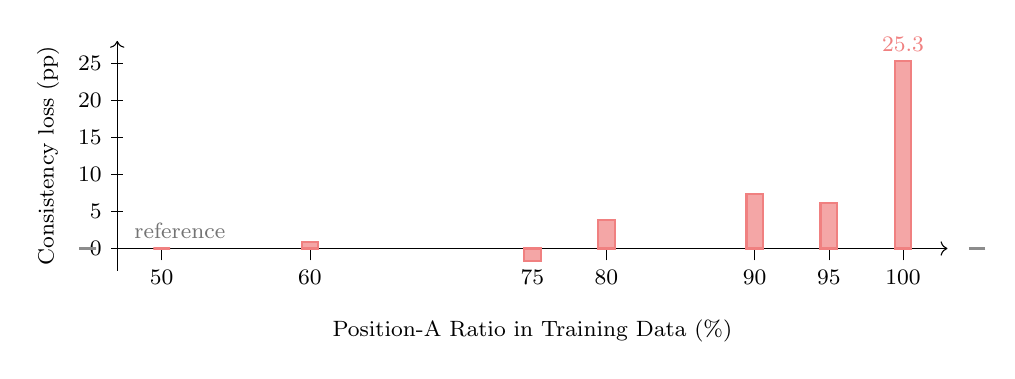
\begin{tikzpicture}
\begin{axis}[
    expplot,
    height=4.5cm,
    xlabel={},
    ylabel={Consistency loss (pp)},
    xmin=47, xmax=103,
    ymin=-3, ymax=28,
    xtick={50,60,75,80,90,95,100},
    xticklabels={50,60,75,80,90,95,100},
    ytick={0,5,10,15,20,25},
    grid=none,
    axis x line=middle,
    axis y line=left,
    axis line style={->},
    x axis line style={yshift=0pt},
    clip=false,
    ybar,
    bar width=6pt,
]
\addplot[black!45, dashed, forget plot] coordinates {(45,0) (105,0)};
\addplot[fill=lr-red!70, draw=lr-red] coordinates {(50,0.0) (60,0.9) (75,-1.7) (80,3.8) (90,7.4) (95,6.1) (100,25.3)};
\node[font=\footnotesize, text=black!55, anchor=south west] at (axis cs:47.5,0) {reference};
\node[font=\footnotesize, text=lr-red, anchor=south] at (axis cs:100,25.3) {25.3};
\node[font=\footnotesize, anchor=north] at (axis description cs:0.5,-0.17) {Position-A Ratio in Training Data (\%)};
\end{axis}
\end{tikzpicture}
\caption{Dose-response as consistency loss from the balanced reference. X ticks are the tested position-A ratios. Bar height is $84.0-\text{consistency}$, so larger bars indicate stronger shortcut damage. The 50\% and 100\% endpoints use multi-seed means; intermediate ratios are single-seed diagnostics.}
\label{fig:dose}
\end{figure}

\section{Threshold Effect Analysis}
\label{app:threshold}

The learning rate sweep shows that shortcut activation exhibits threshold-like behavior rather than smooth degradation (Figure~\ref{fig:lr}). At low learning rates, consistency remains close to the baseline. Once optimization pressure crosses a critical point, original-order accuracy rises while consistency drops sharply, suggesting that the simpler position feature receives enough reward signal to dominate the learned policy.

Cross-model validation on Qwen3-8B is consistent with this interpretation, but the effect is weaker. Qwen3-8B maintains consistency in the high-70s to low-80s across tested learning rates and reaches 78.4\% at the largest rate (Table~\ref{tab:crosslr}), while Qwen2.5-7B collapses at aggressive rates. The shortcut is not eliminated by model capability, but it appears harder to activate. Practitioners using newer, stronger models may not observe the problem at standard learning rates, yet it can still emerge with hyperparameter changes.

\bibliography{custom}

\end{document}
